\chapter{Resultados}
\label{cap:resultados}

\section{Tamaños y tiempos}
Lo primero que debemos considerar como resultado, es el tiempo de ejecución de la aplicación, ya que nos encontramos ante un dispositivo movil, que no dispone de la misma cantidad de recursos que un ordenador portatil o de sobremesa.\\

También hay que tener en cuenta que estamos trabajando con imágenes, por lo que a mayor cantidad de píxeles de esta, mayor será el tiempo de cómputo, por lo que se debe encontrar un equilibrio entre el tamaño de las imagénes y el resultado obtenido. De nada nos sirve que la aplicación tarde muy poco tiempo en comparar un gran número de imágenes si el resultado es totalmente erroneo.\\

En una serie de pruebas iniciales, el tamaño de las imágenes no se tuvo en cuenta, por lo que incluso con el descriptor prototipo, no realizaba níngún tipo de cálculo, los tiempos de consulta eran demasiado elevados, a pesar de usar un número pequeño de imágenes.\\

El siguiente paso fue redimensionar las imágenes a un tamaño concreto, se comenzó con 200x200. Con este tamaño se redujo el tiempo de cómputo, y los resultados comenzaban a ser prometedores. Pero se comprobó que el tiempo de cómputo crecía demasiado con el número de imágenes, por lo que se descartó este tamaño.\\

Con los tamaños 64x64 y 32x32, este último es el definitivo, se obtuvieron unos buenos tiempos de ejecución y unos buenos resultados, aunque se decidió usar 32x32 ya que el descriptor MPEG7, realiza una gran cantidad de operaciones con el histograma de la imagen, por lo que ese tamaño se adapta mejor a nuestras necesidades. Se probaron estos dos últimos tamaños, ya que en una asignatura de este máster se tuvo que trabajar con imágenes, y dichos tamaños, son los que mejores resultados nos proporcionaron.\\

\section{Consultas}

Una vez discutidos los tiempos y tamaños, es hora de comprobar que los resultados de las consultas son los esperados. Para ello vamos a utilizar dos bases de imágenes:\\

\begin{itemize}

\item Banderas. Un cojunto de 160 con las banderas de los principales países del mundo.

\item VisTex. Conjunto de imágenes de texturas, constituida por un total de 669 elementos.

\end{itemize}

\begin{figure}[H] %con el [H] le obligamos a situar aquí la figura
\centering
\includegraphics[scale=0.5]{imagenes/banderas.png}  %el parámetro scale permite agrandar o achicar la imagen. En el nombre de archivo puede especificar directorios
\label{banderas}
\caption{Base de datos de banderas}
\end{figure}

\begin{figure}[H] %con el [H] le obligamos a situar aquí la figura
\centering
\includegraphics[scale=0.5]{imagenes/texturas.png}  %el parámetro scale permite agrandar o achicar la imagen. En el nombre de archivo puede especificar directorios
\label{texturas}
\caption{Base de datos de VisTex}
\end{figure}

Como es natural, también se han realizado las pruebas con imágenes propias de mi dispositivo, pero por comodidad y para ver mejor los resultados se ha decidido usar estas dos bibliotecas.


\subsection{SingleColorDescription}

Este descriptor se basa en el cálculo del color medio de la imagen encontrándose esta, en un espacio de color RGB. Por lo que las imágenes con colores más parecidos aparecerán juntas.

Ahora vamos a comentar una consulta utilizando este descriptor y VisTex:

\begin{figure}[H] %con el [H] le obligamos a situar aquí la figura
\centering
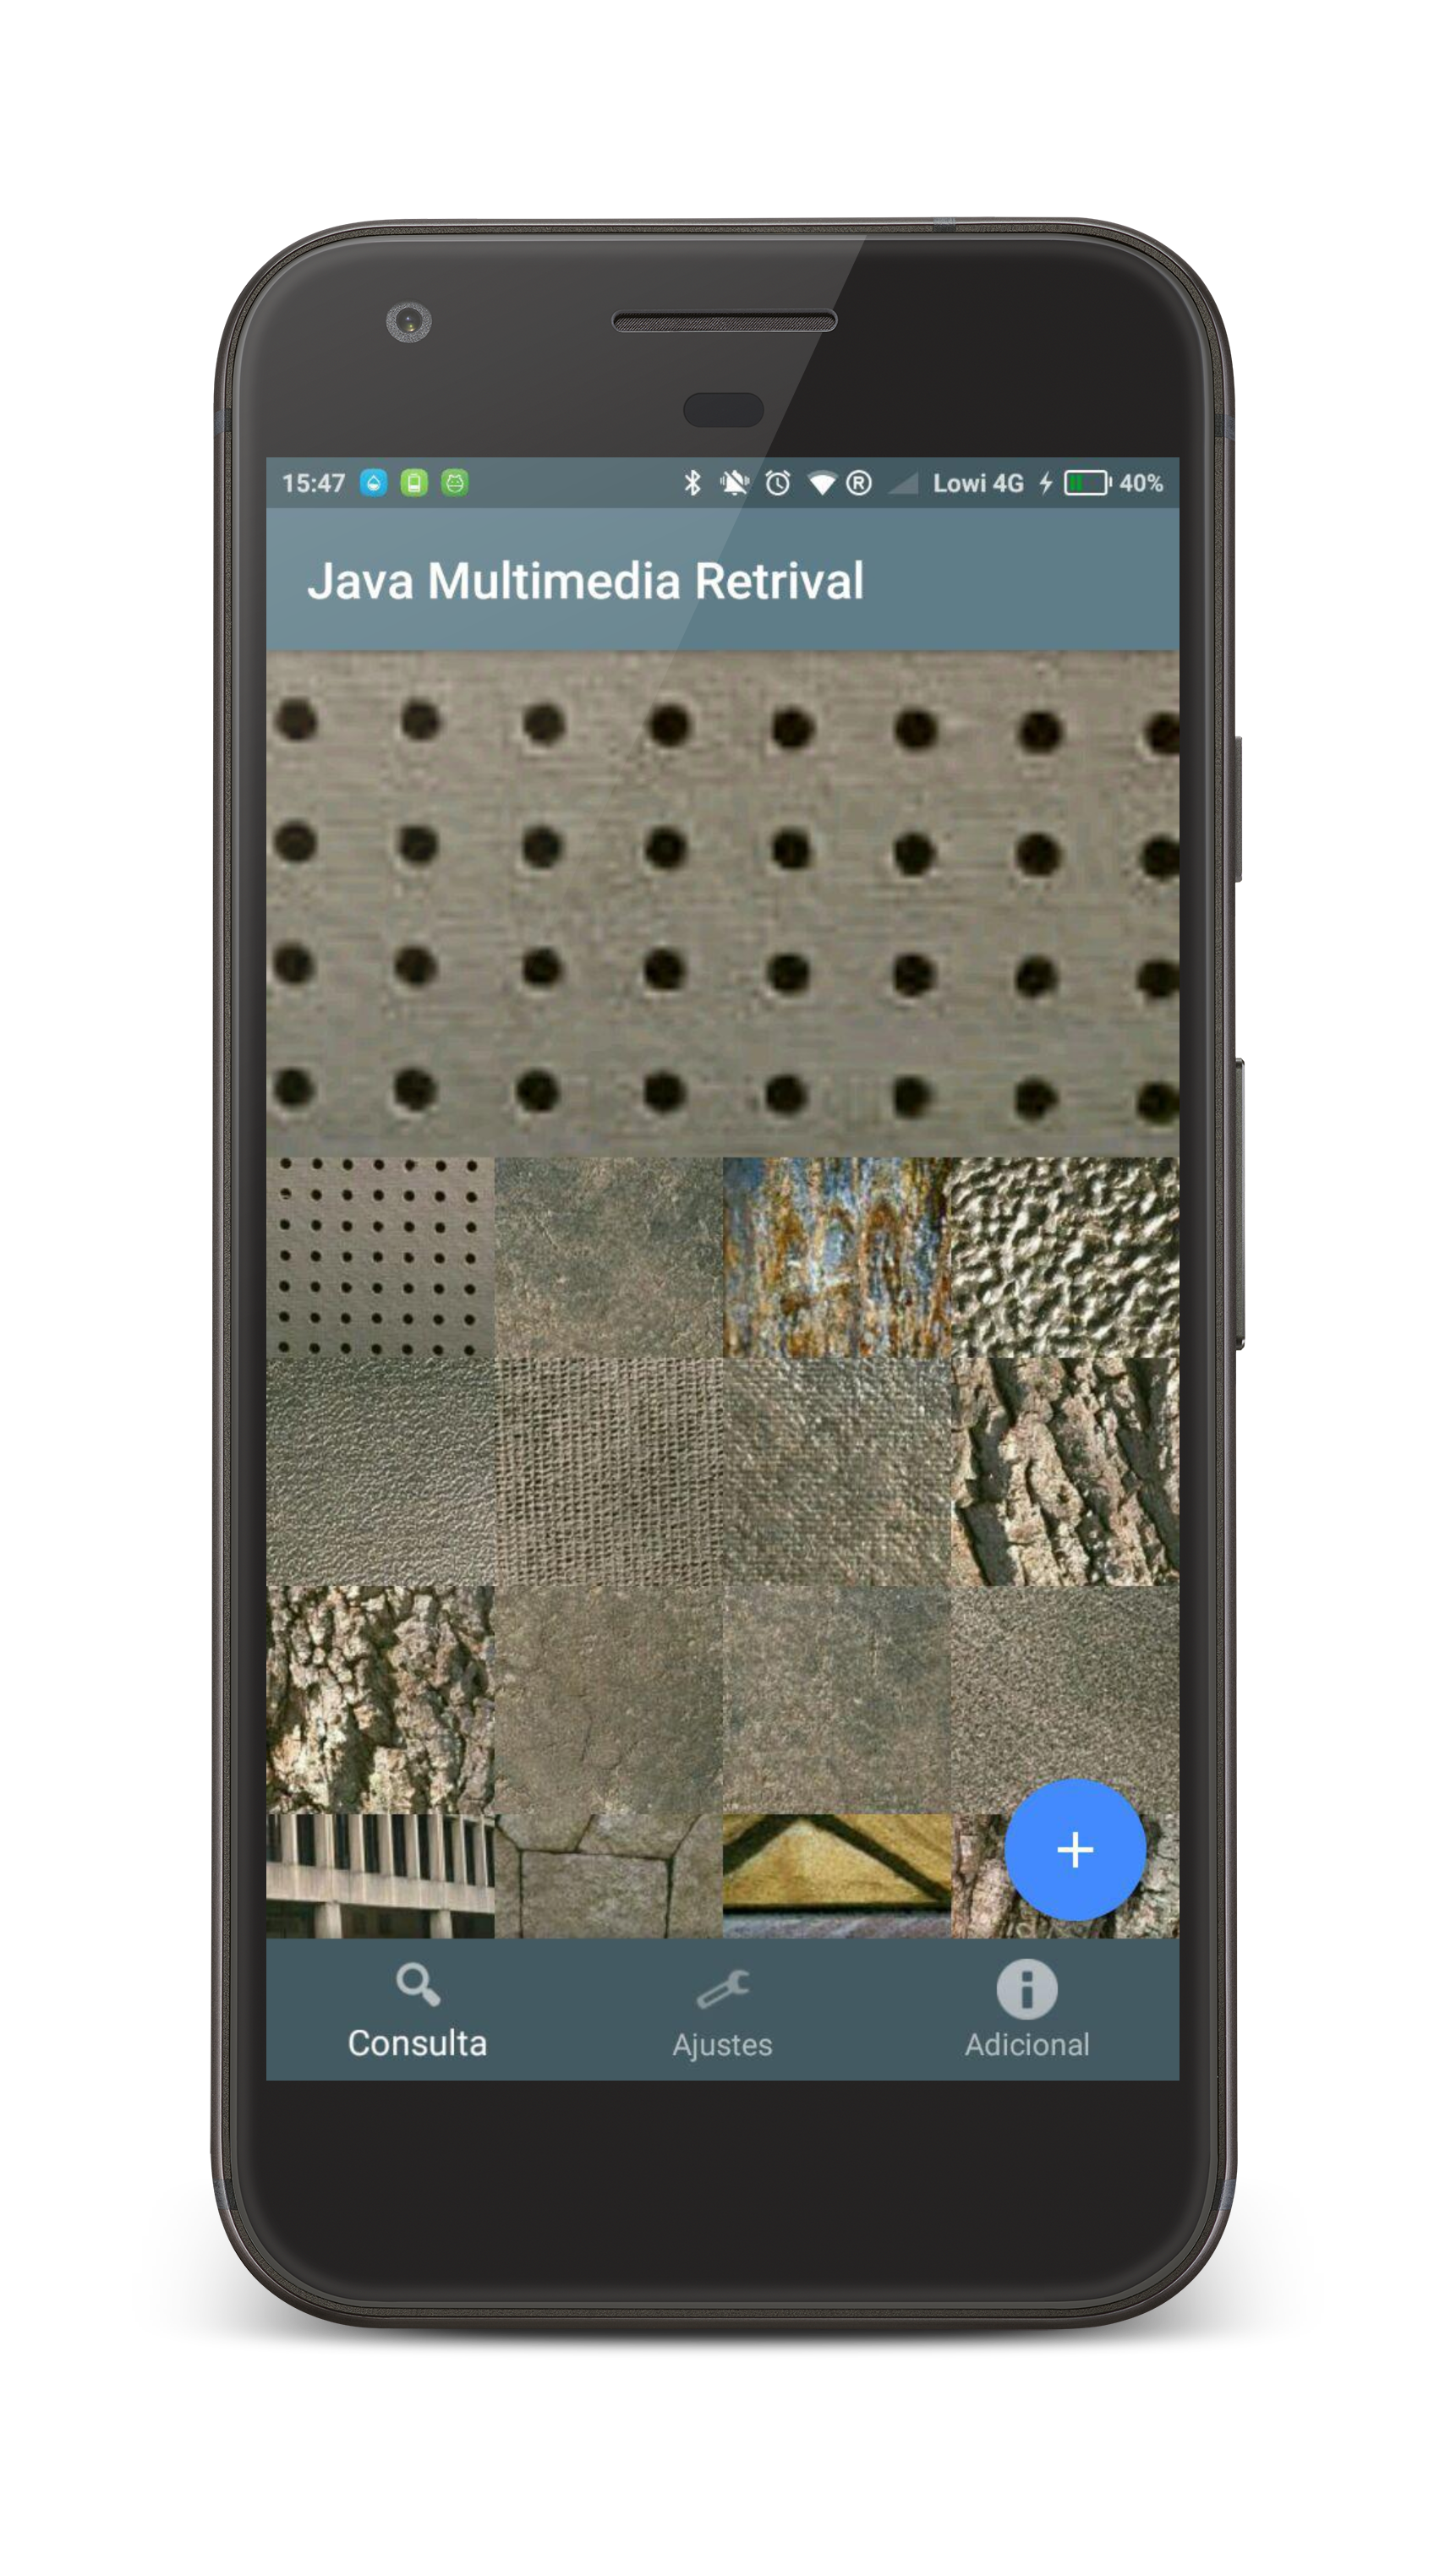
\includegraphics[scale=0.15]{imagenes/SingleColorresultado1.png}  %el parámetro scale permite agrandar o achicar la imagen. En el nombre de archivo puede especificar directorios
\label{SingleColorresultado1.png}
\caption{Resultado consulta SingleColorDescriptor 1 }
\end{figure}

\begin{figure}[H] %con el [H] le obligamos a situar aquí la figura
\centering
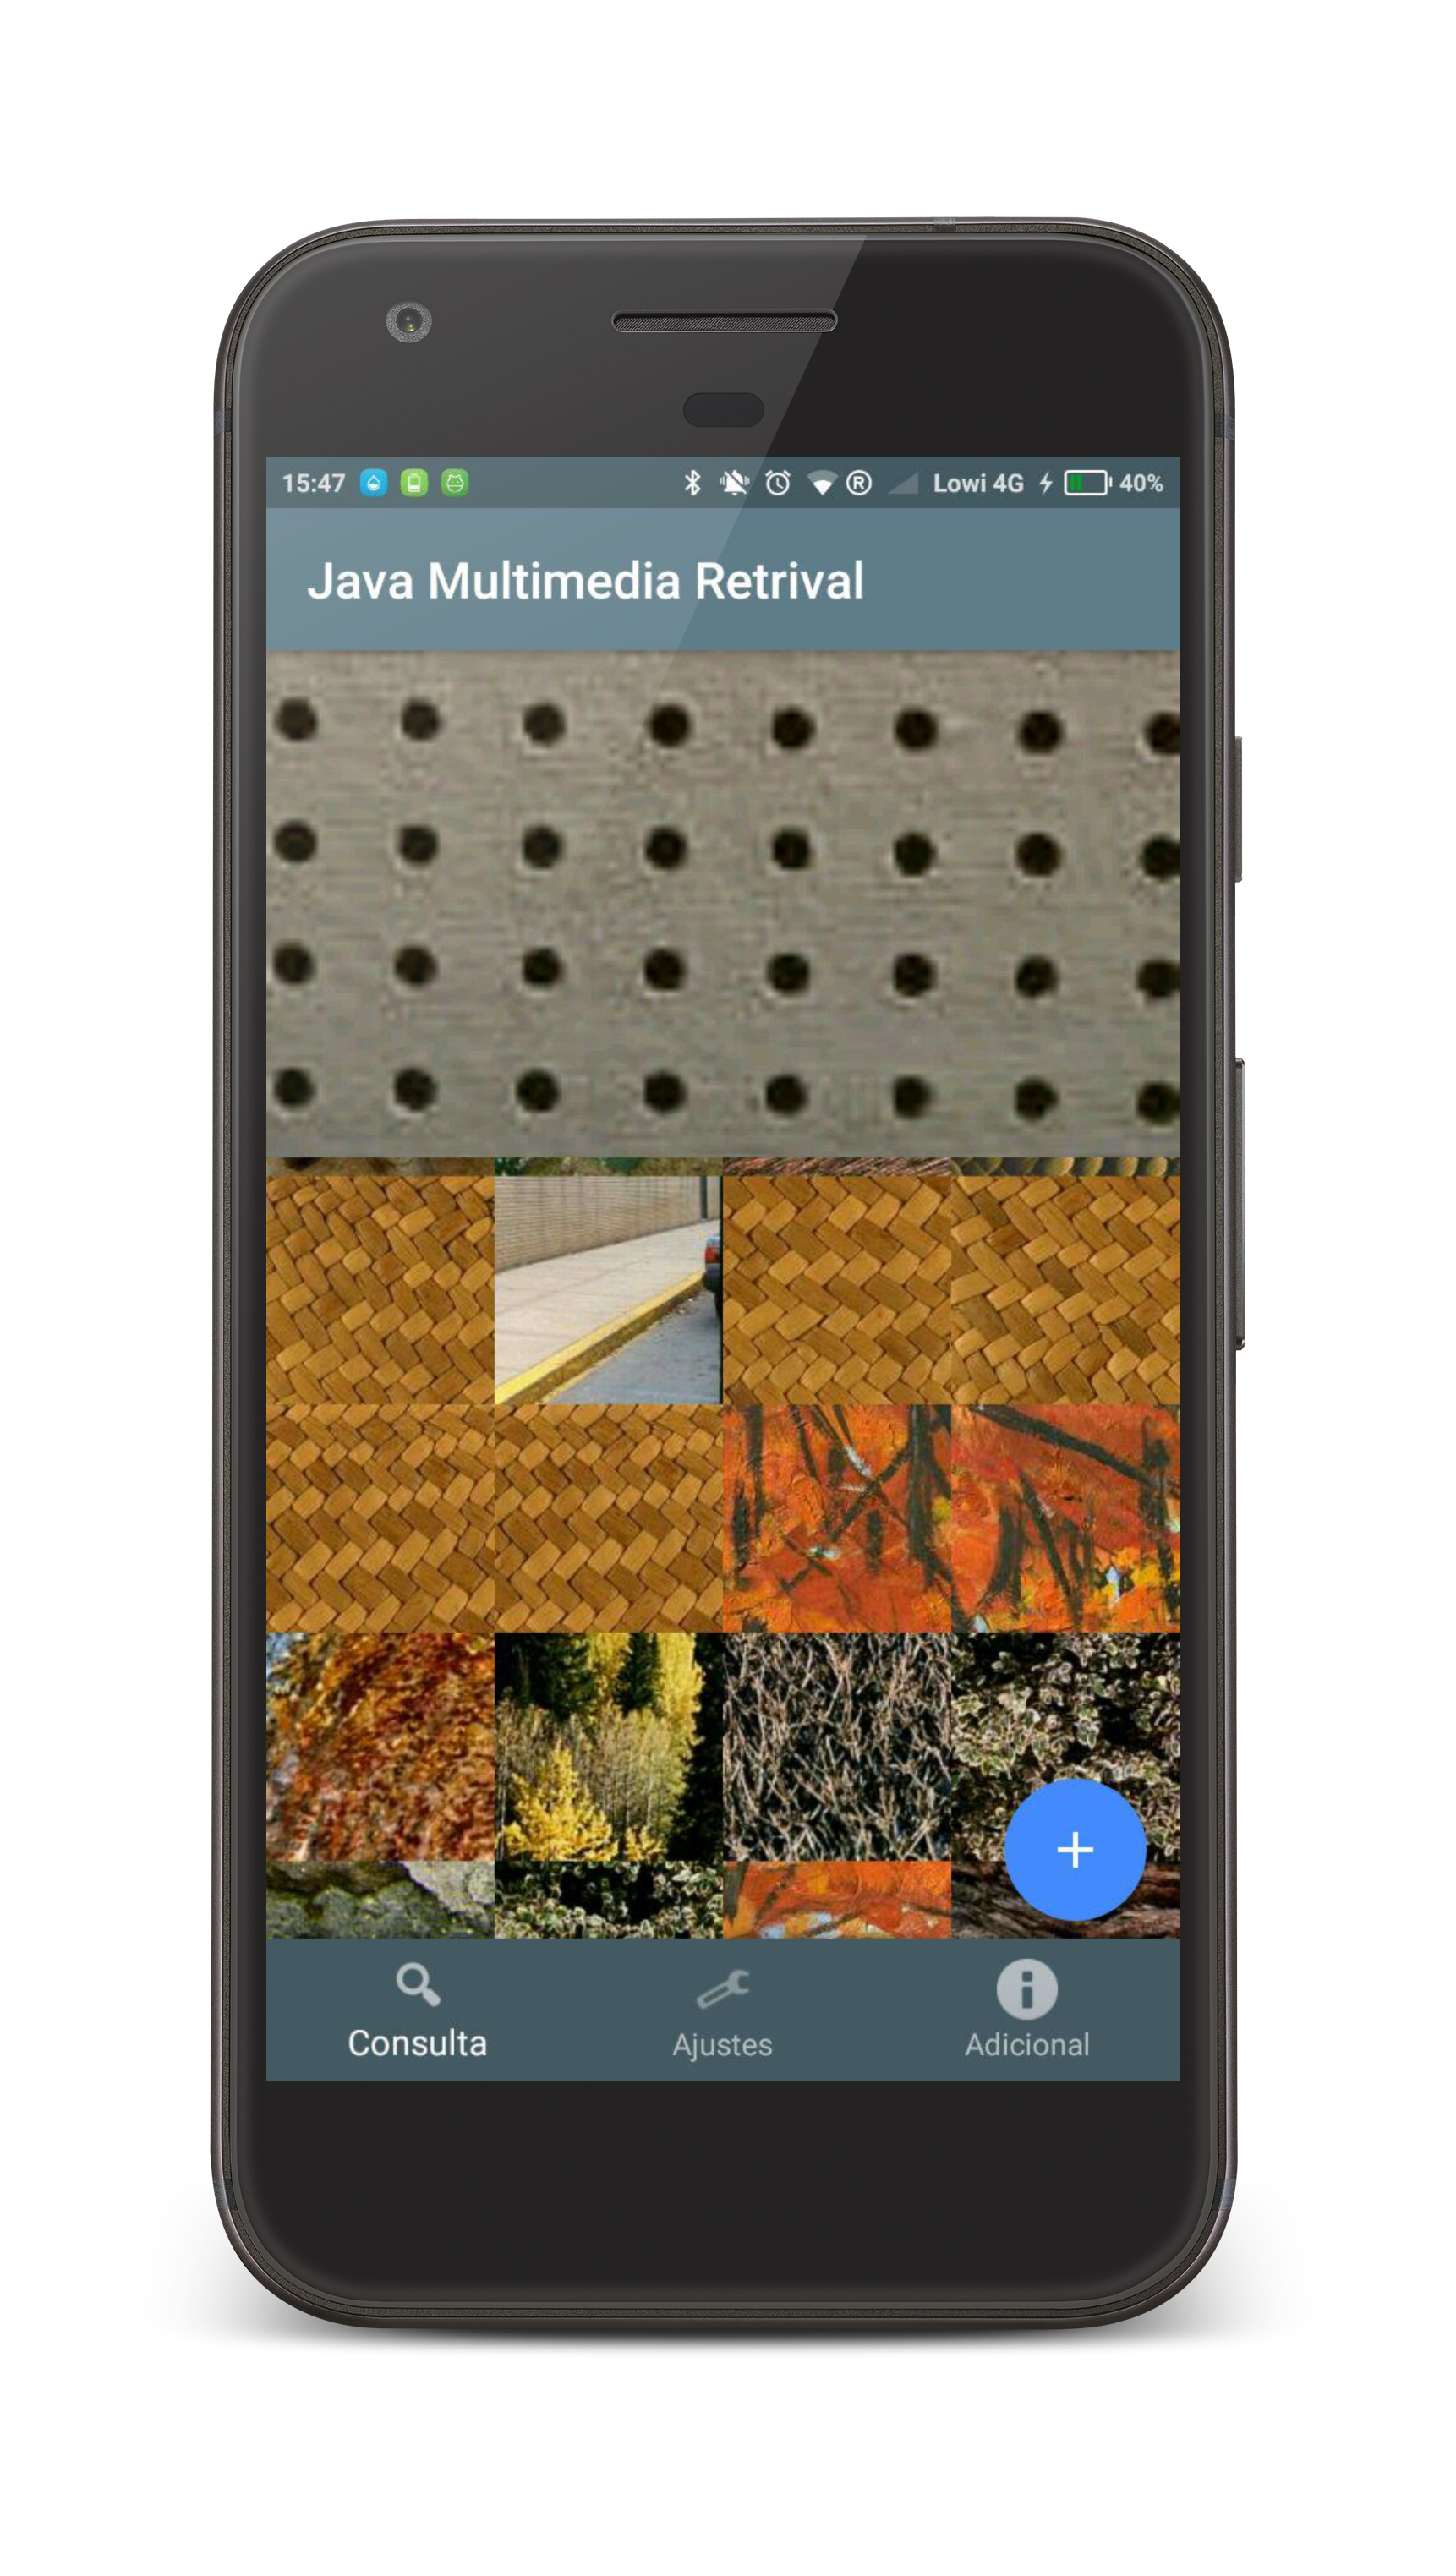
\includegraphics[scale=0.15]{imagenes/SingleColorresultado2.png}  %el parámetro scale permite agrandar o achicar la imagen. En el nombre de archivo puede especificar directorios
\label{SingleColorresultado2.png}
\caption{Resultado consulta SingleColorDescriptor 2 }
\end{figure}

Podemos comprobar como en la primera imagen, que sería lo primero que veríamos al realizar una consulta, las imágenes resultado, son muy parecidas en color a la imagen original. Por otro lado, en la segunda imagen se aprecian imágenes que se parecen menos a la consulta, por lo que se encuentran en posiciones más alejadas. Para llegar a ellas podemos usar el movimiento de scroll.


\subsection{MPEG7ColorStructure}

El descriptor MPEG7ColorStructure se basa en el cálculo del histograma empleando imágenes en el espacio de color HMMD. Los resultados serían parecidos a los del descriptor anterior.

\begin{figure}[H] %con el [H] le obligamos a situar aquí la figura
\centering
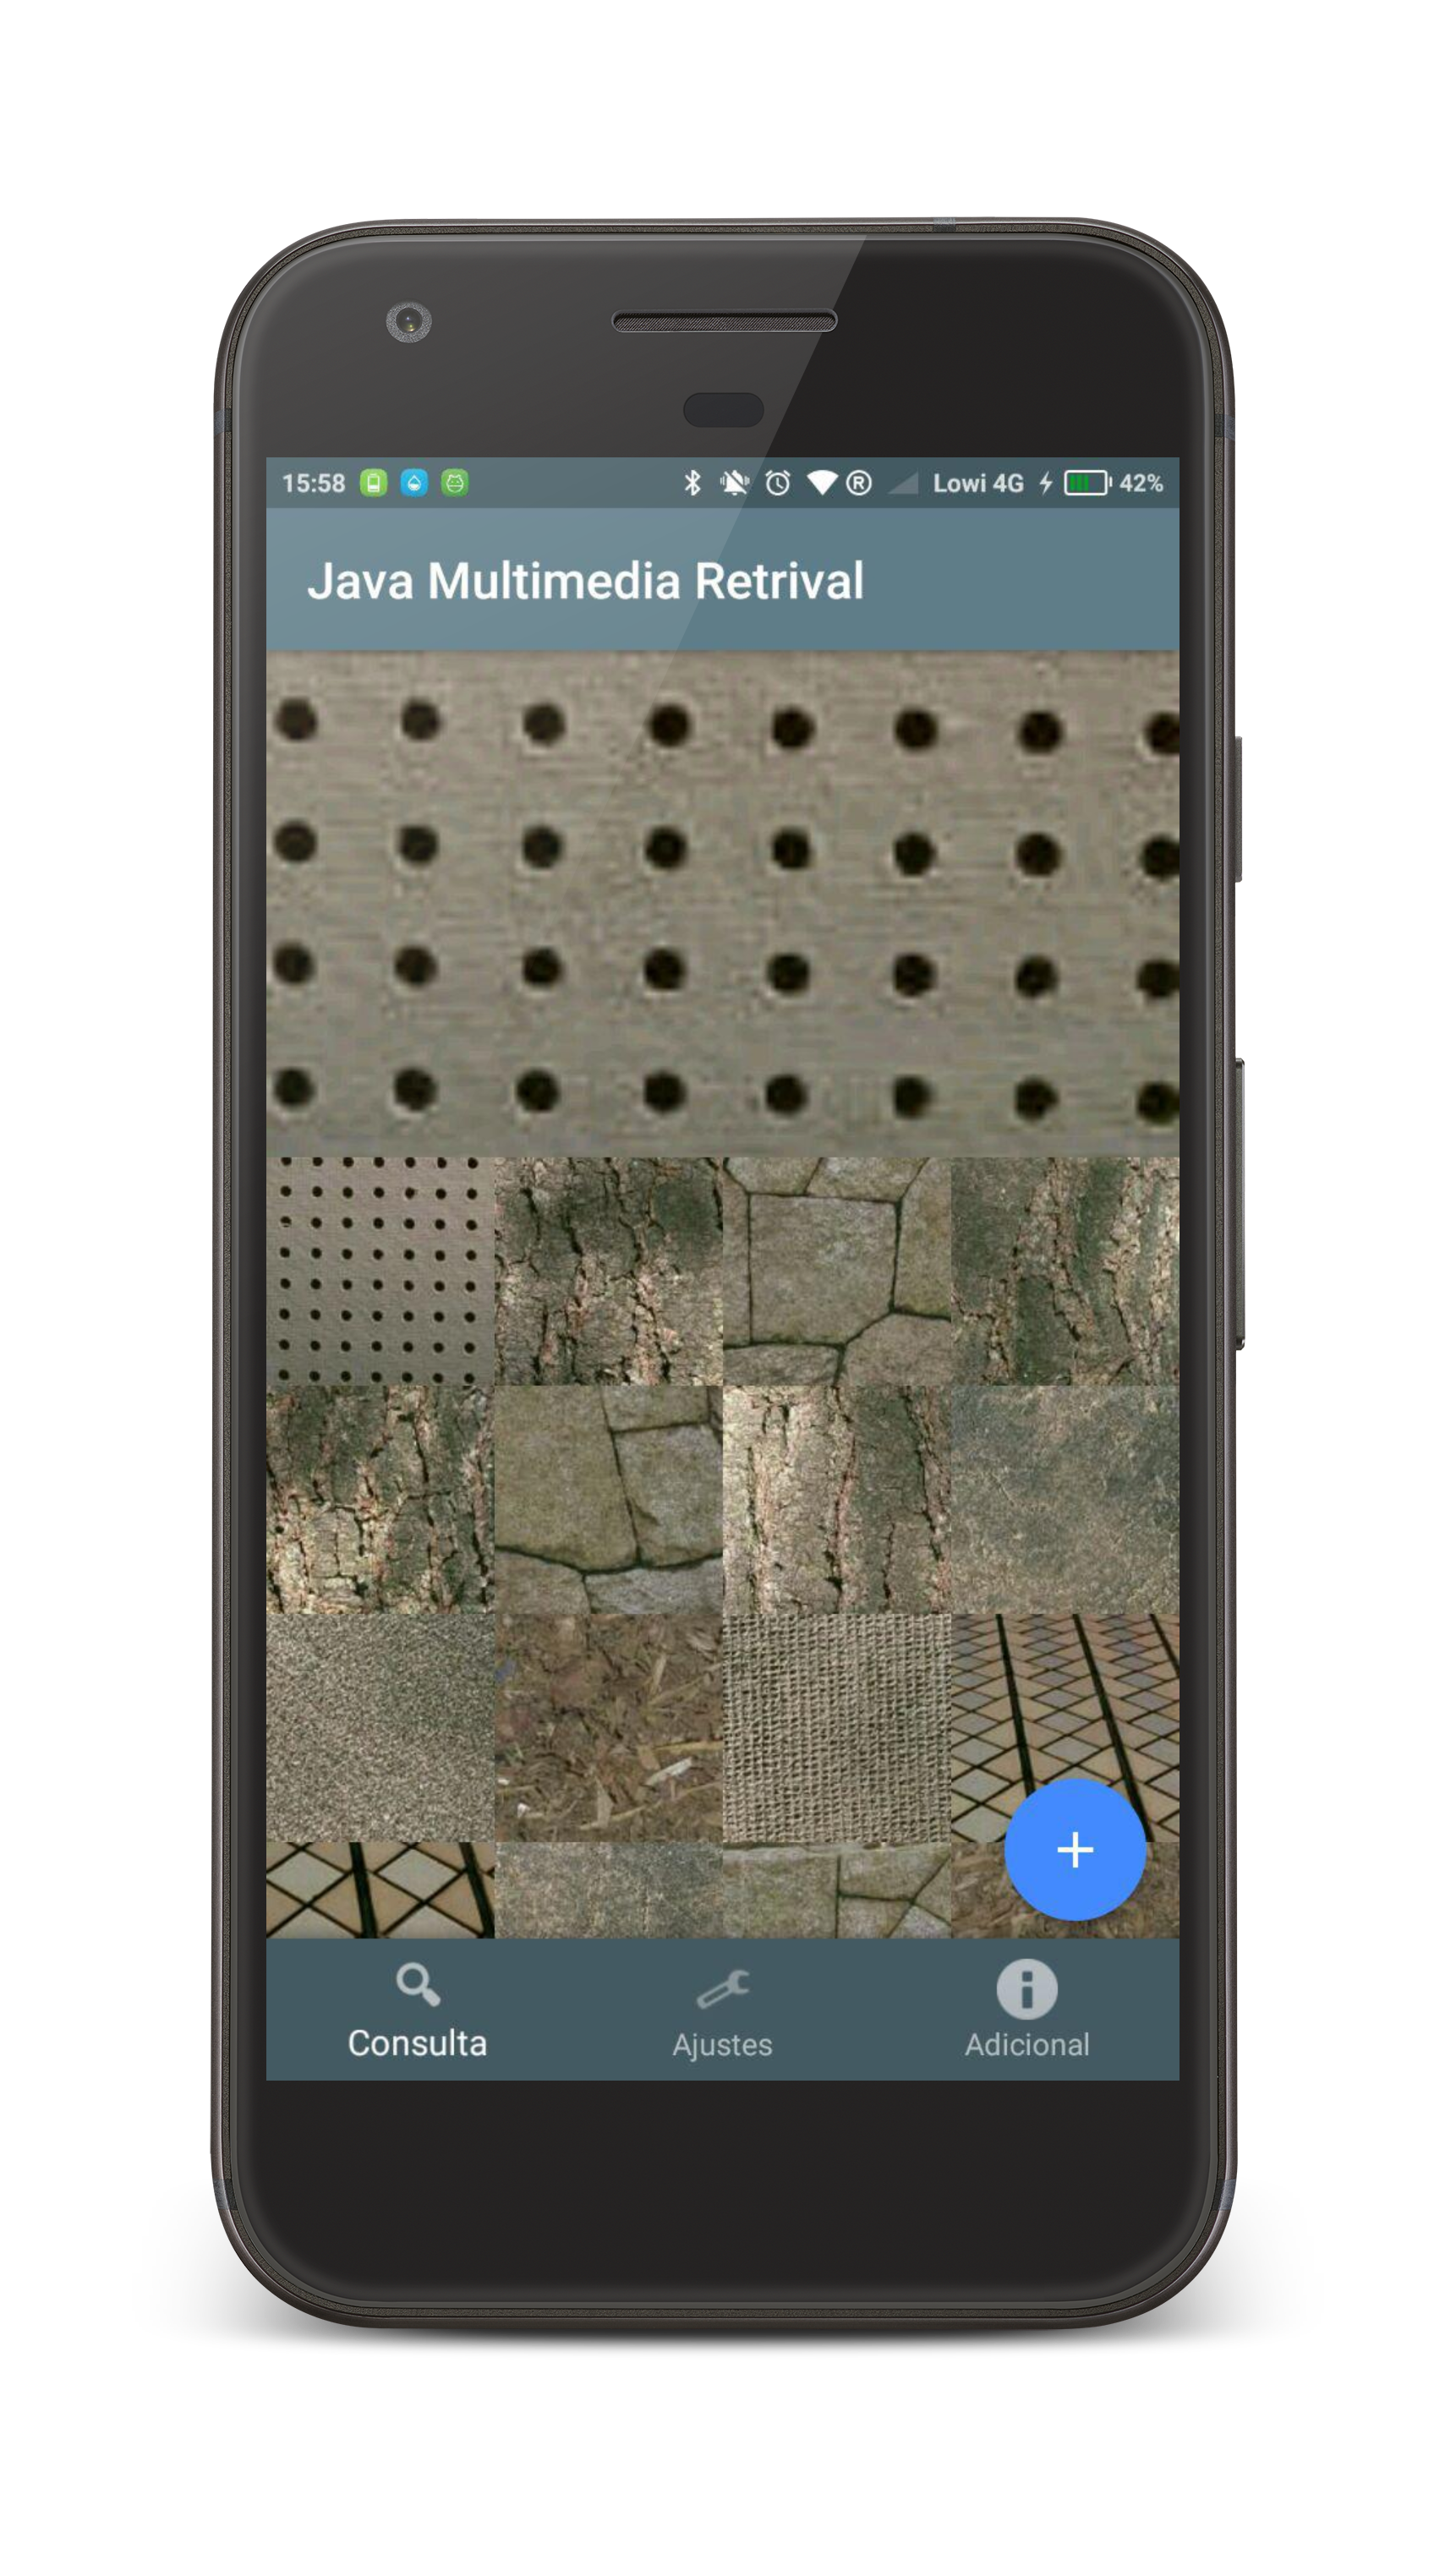
\includegraphics[scale=0.15]{imagenes/mpegResultado1.png}  %el parámetro scale permite agrandar o achicar la imagen. En el nombre de archivo puede especificar directorios
\label{mpegResultado1.png}
\caption{Resultado consulta SingleColorDescriptor 1 }
\end{figure}

\begin{figure}[H] %con el [H] le obligamos a situar aquí la figura
\centering
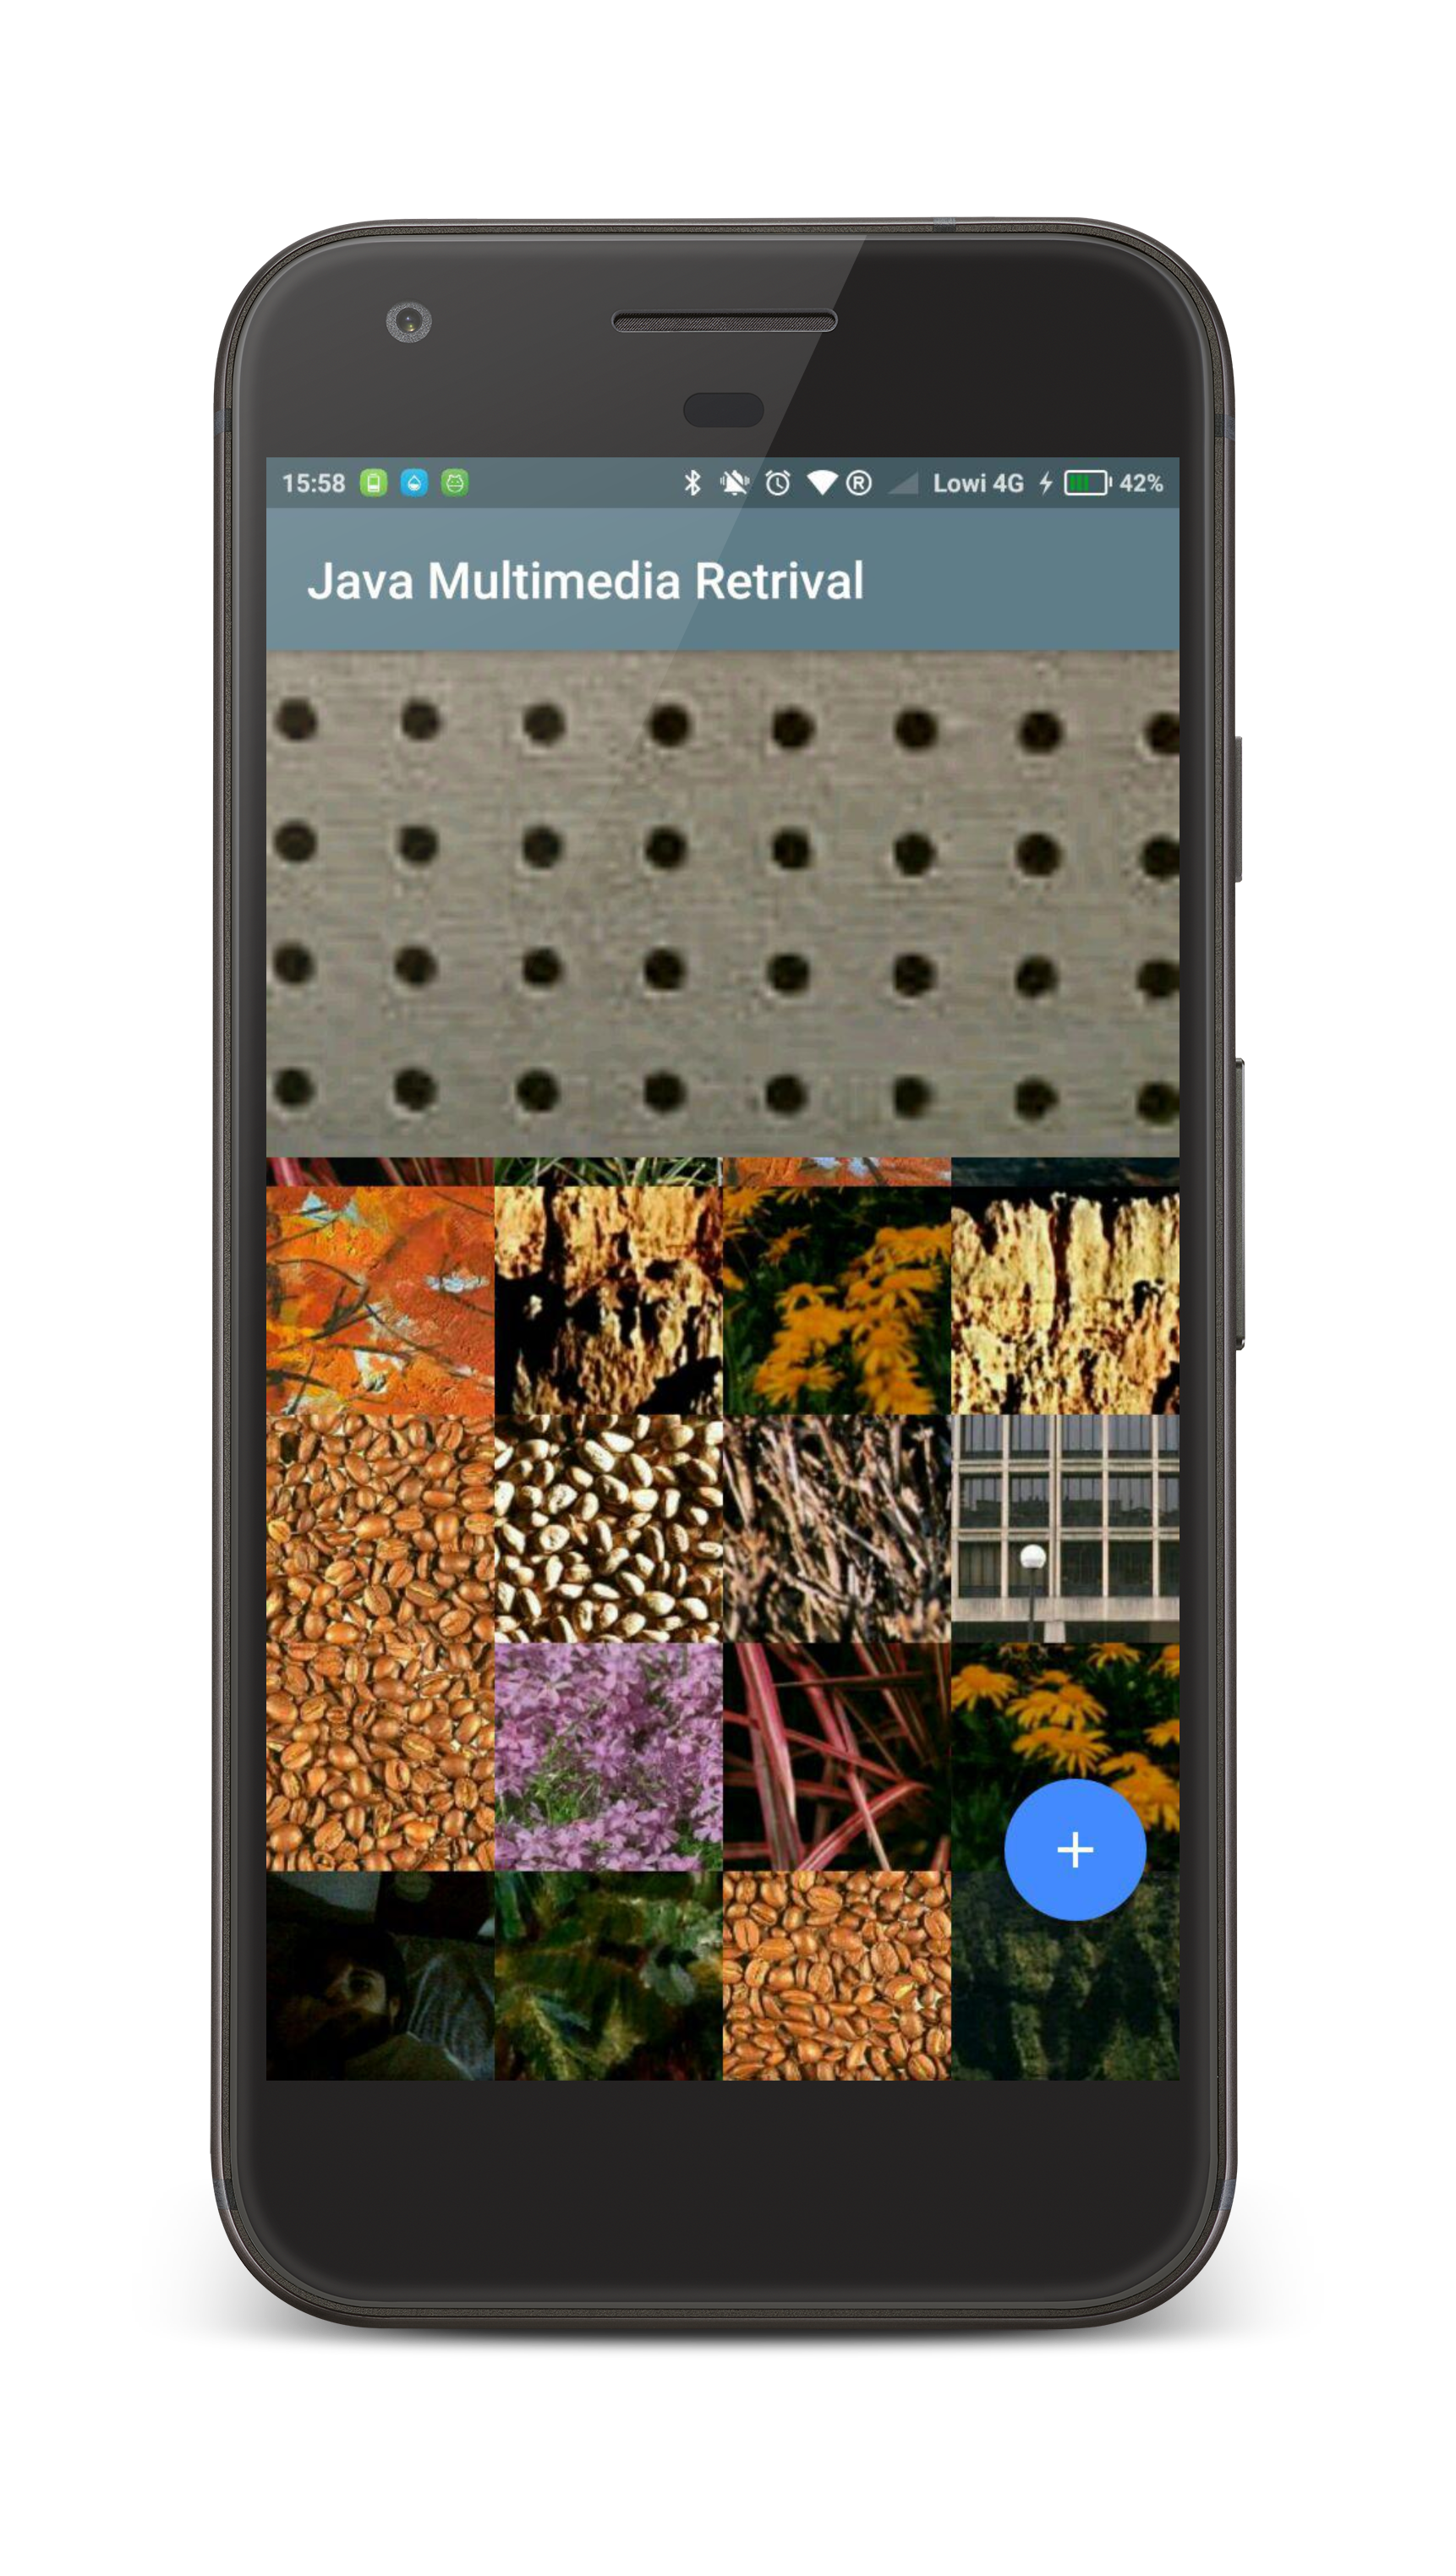
\includegraphics[scale=0.15]{imagenes/mpegResultado2.png}  %el parámetro scale permite agrandar o achicar la imagen. En el nombre de archivo puede especificar directorios
\label{mpegResultado1.png}
\caption{Resultado consulta SingleColorDescriptor 2 }
\end{figure}

Se puede ver como este descriptor obtiene mejores resultados. Las primeras imágenes resultado son más uniformes, mientras que en el caso anterior, habia un mayor número de diferencias. Y por otro lado, como se agrupan mejor las imágenes menos parecidas.





